\chapter{Conception}


\section{Introduction}
Les activités d'expression des besoins et d'analyse ont permis de définir quel système a construire.

L’activité de conception s’intéresse à la façon de construire le système, elle propose donc une solution qui doit satisfaire aux besoins du système, une décomposition modulaire y est souvent recommandée.

L’architecture du logiciel ainsi que chacun de ses constituants: informations traitées, traitements effectués, résultats fournis, contraintes à respecter.La conception orientée objet (COO) consiste à concevoir l’organisation des modules (classes) du logiciel et du stockage des données persistantes.

\begin{itemize}
	\item La conception constitue un point de départ à l’implémentation 
	\item décompose le travail d’implémentation en sous-systèmes.
	\item crée une abstraction transparente de l’implémentation. 
\end{itemize}

\section{Modèle du domaine}
Le diagramme de classes en montre la structure interne. Il permet de fournir une représentation abstraite des objets du système qui vont interagir ensemble pour réaliser les cas d’utilisation. Il est important de noter qu’un même objet peut très bien intervenir dans la réalisation de plusieurs cas d’utilisation.

\begin{figure}[H]
	\centering
	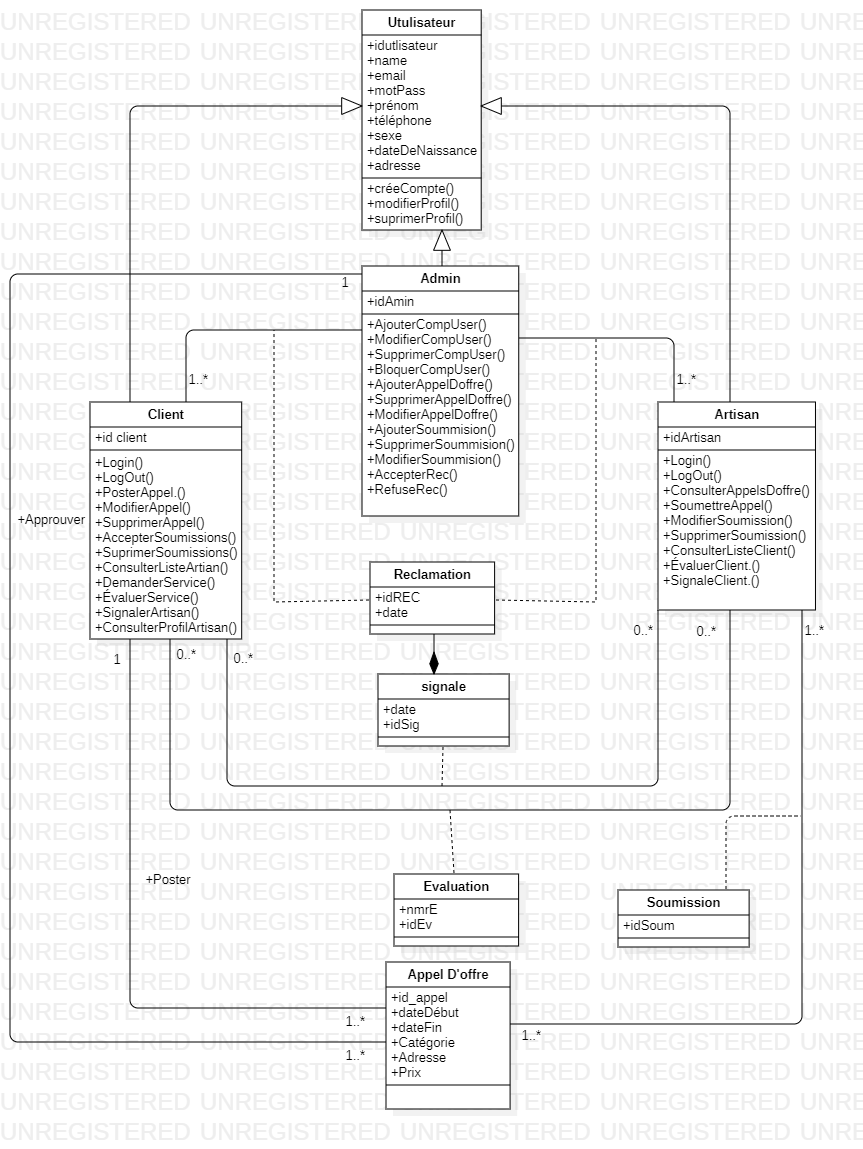
\includegraphics[scale=0.5]{DiagrammeDeClasse.png}
	\caption{Diagramme de classe}
	\label{fig:diagramme class}
\end{figure}

\section{Diagrammes d’activité}
Les diagrammes d’activités sont également utiles dans la phase de réalisation car ils permettent une description si précise des traitements qu’elle autorise la génération automatique du code.

\subsection{Modifier Profil}

\begin{figure}[H]
	\centering
	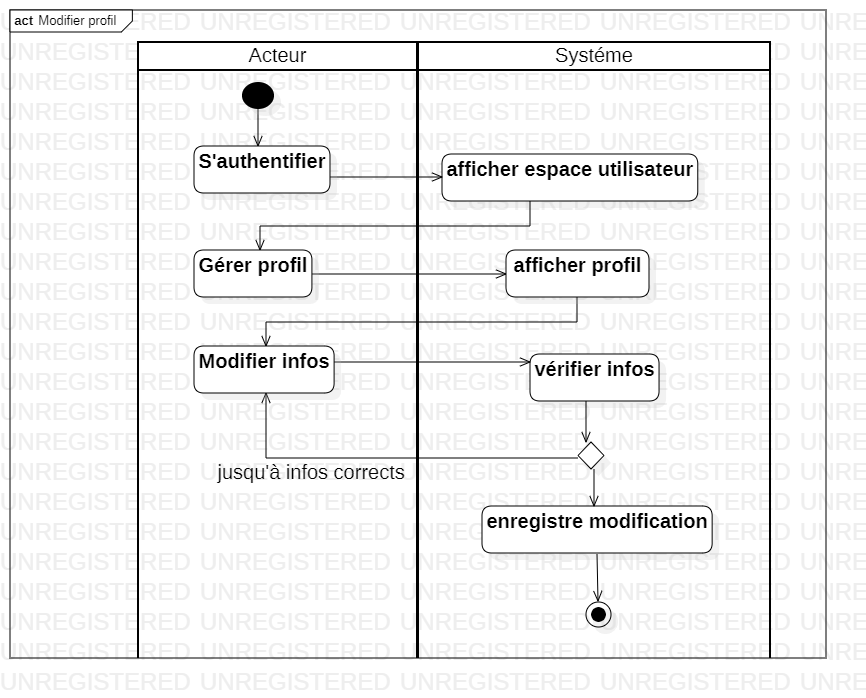
\includegraphics[scale=0.5]{CliModifierProfil.png}
	\caption{Diagramme d'action Modifier Profil}
	\label{fig:action modifier profil}
\end{figure}

\subsection{Poster Un appel d'offre}

\begin{figure}[H]
	\centering
	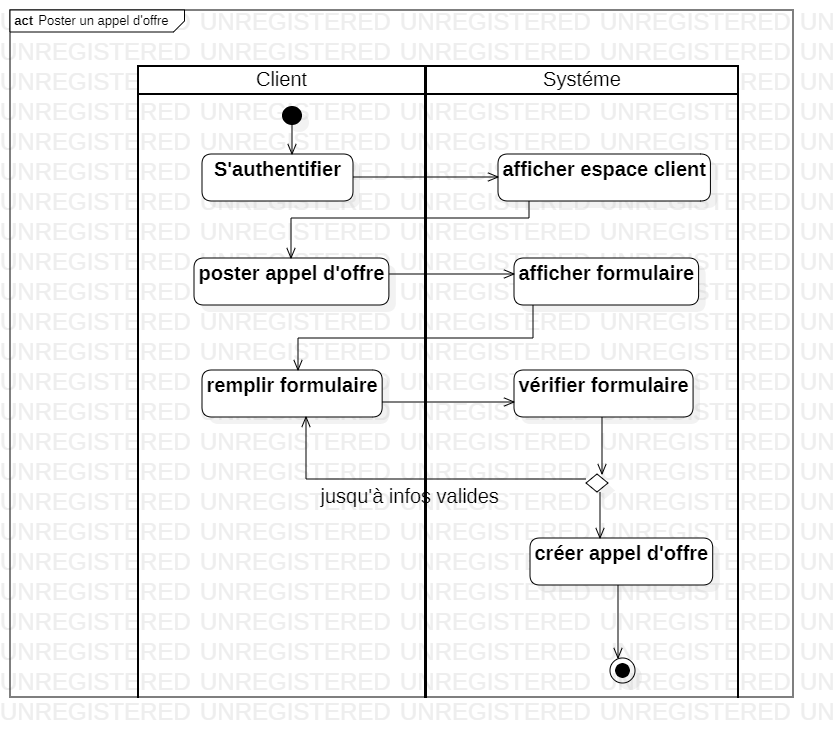
\includegraphics[scale=0.5]{CliPosterAppel.png}
	\caption{Diagramme d'action Poster Appel}
	\label{fig:action poster appel}
\end{figure}

\subsection{Signaler}

\begin{figure}[H]
	\centering
	
\includegraphics[scale=0.5]{signaler.png}
	\caption{Diagramme d'action signaler}
	\label{fig:action signaler}
\end{figure}

\subsection{Soumettre appel d’offre}

\begin{figure}[H]
	\centering
	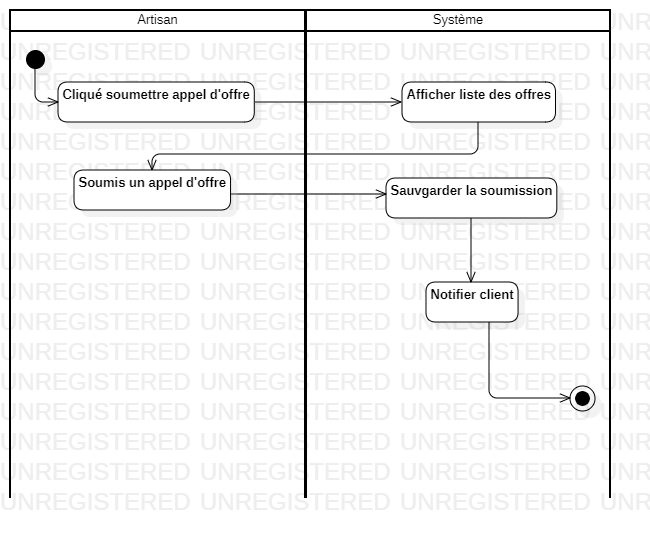
\includegraphics[scale=0.5]{Soumettre appel d'offre.png}
	\caption{Diagramme d'action Soumettre appel d'offre}
	\label{fig:action soumettre appel d'offre}
\end{figure}

\subsection{Bloquer Utilisateur}

\begin{figure}[H]
	\centering
	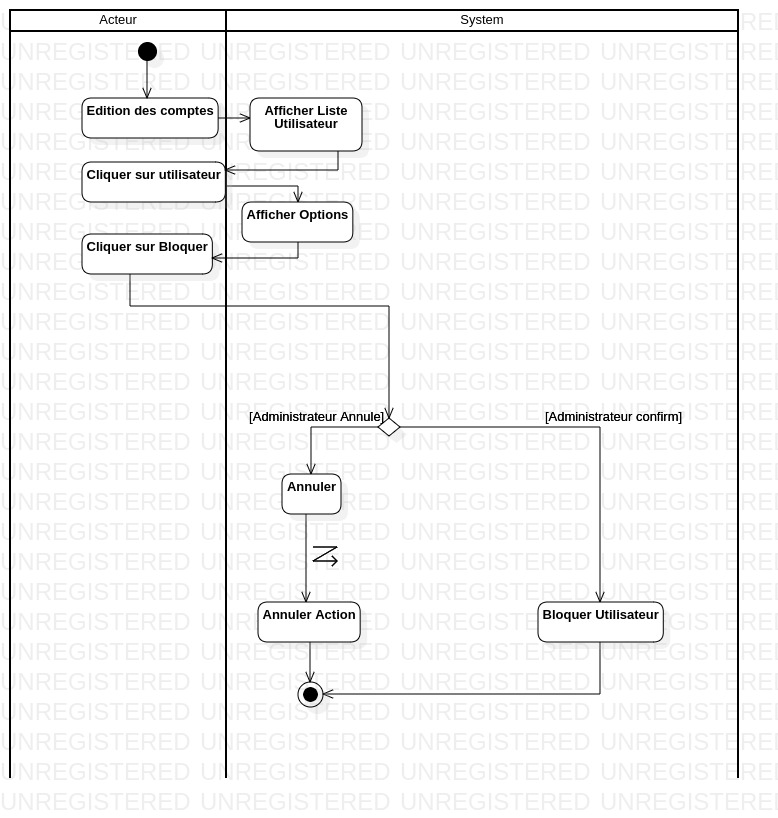
\includegraphics[scale=0.5]{BloquerUtilisateurAction.jpg}
	\caption{Diagramme d'action Bloquer utilisateur}
	\label{fig:action bloquer user}
\end{figure}

\subsection{Gérer Réclamation}

\begin{figure}[H]
	\centering
	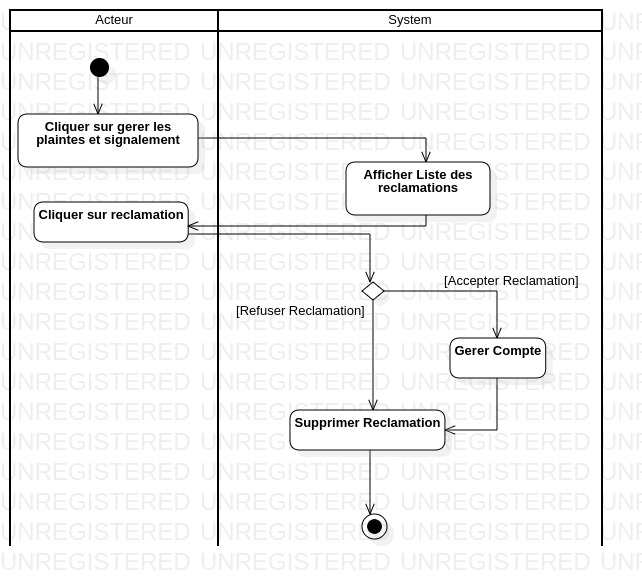
\includegraphics[scale=0.5]{GereReclamationAction.jpg}
	\caption{Diagramme d'action Gérer réclamations}
	\label{fig:action gerer reclamation}
\end{figure}

\section{Schéma de base de données}
\subsection{Règles de passages}
\begin{enumerate}
	\item Transformation des classes: Les classes dans un diagramme de classes sont transformées aux des relations dans  modèle relationnelle dans la base de données et des tables dans le modèle physique .
	
	\item Transformation des attributs : Les attributs des classes dans un diagramme de classes sont considérés comme des attributs pour les relations dans le modèle relationnel dans la base de données et des colonnes dans les tables dans le modèle physique .
	L’identifiant de classe est transformé en une clé primaire dans la BD .
	
	\item Transformation des associations : 
		\subitem Association de 1 à N : Pour chaque classe A de diagramme , elle a une association de 1 à N avec classe B , il faut ajouter l’identifiant de la classe B - clé primaire dans BD - comme un clé étrangère dans BD .
		
		\subitem Association de 1: Il existe deux solutions :
		\begin{itemize}
			\item Si les deux multiplicités minimales sont à un, il est préférable de fusionner les deux classes en une seule .
			\item Sinon on fait la même chose pour une association de 1 à N .
		\end{itemize}
	
		\subitem Association de 0 à N: Chaque classe-association est représentée par une relation. La clé primaire de cette relation est la concaténation des identifiants - clés primaires-  des classes connectées à l'association
		
	\item Transformation des compositions: Chaque élément de la classe composite est représenté par une relation , il faut ajouter l’identifiant - clé primaire -   de cette classe comme un clé étrangère à l'élément de la composite.
	
	\item Transformation d'héritage: Chaque classe mère ou fille est représentée par une relation . L’identifiant - clé primaire - de la classe mère est ajouté comme un clé primaire et clé étrangère à la fois dans la classe fille.
	
\end{enumerate}

\subsection{Les relations de la base de données}

\noindent Utilisateur ( \underline{idUtilisateur} , nome , prénom , email , motPasse , téléphone , sexe , dateNaissance , adresse )\\
Admin ( \underline{idAdmin} , \#idUtilisateur )\\
Client ( \underline{idClient} , \#idUtilisateur )\\
Signale ( \underline{idSignale} , date , \#idClient , \#idArtisan )\\
Réclamation ( \underline{idReclamation} , description , \#idSignale , \#idClient , \#idAdmin , \#idArtisan )\\
Evaluation ( \underline{idEvaluation} , nmrEvaluation , \#idClient ,\#idArtisan )\\
Soumissions ( \underline{idSoumissions} , description , \#idAppel , \#idArtisan )\\
Appel d’offre ( \underline{idAppel} , dateDébut , dateFin , catégorie ,  prix , adresse ,\#idClient , \#idArtisan , \#idAdmin )\\

\begin{figure}[H]
	\centering
	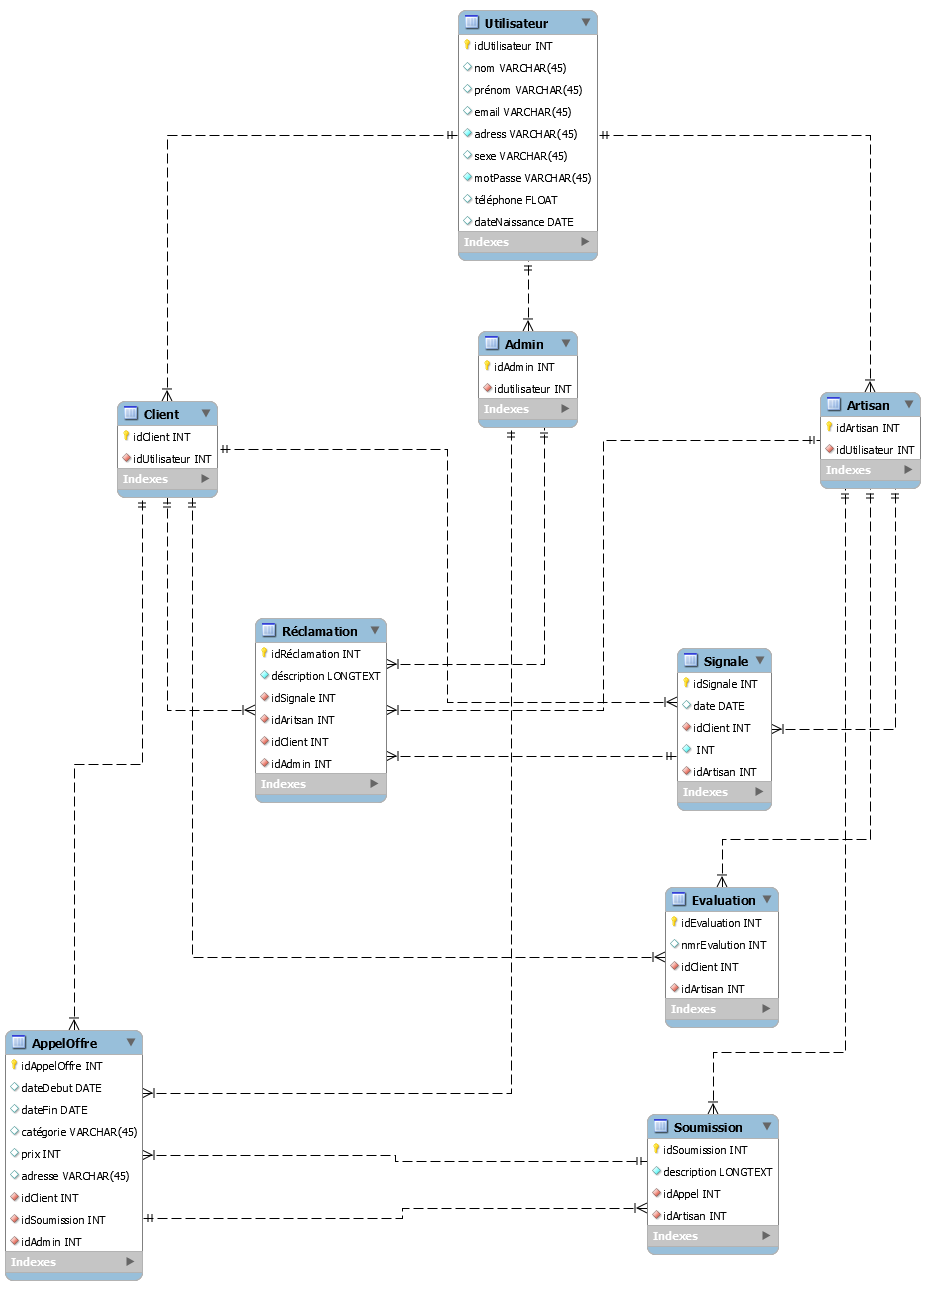
\includegraphics[scale=0.5]{SchemaDB.png}
	\caption{Schéma Base de donnée}
	\label{figure: scheme bd}
\end{figure}

\section{Conclusion}
Durant ce chapitre nous avons , nous avons détailler notre projet, nous avons réalisé une analyse profonde de la solution adaptée en précisant les différentes fonctionnalités du système 